\documentclass[border=10pt]{standalone}

\usepackage{tikz}
\usepackage{tikzsymbols}
\usetikzlibrary{calc,patterns,shapes.geometric}

\def\centerarc[#1](#2)(#3:#4:#5){\draw[#1] ($(#2)+({#5*cos(#3)},{#5*sin(#3)})$) arc (#3:#4:#5);}

\begin{document}
	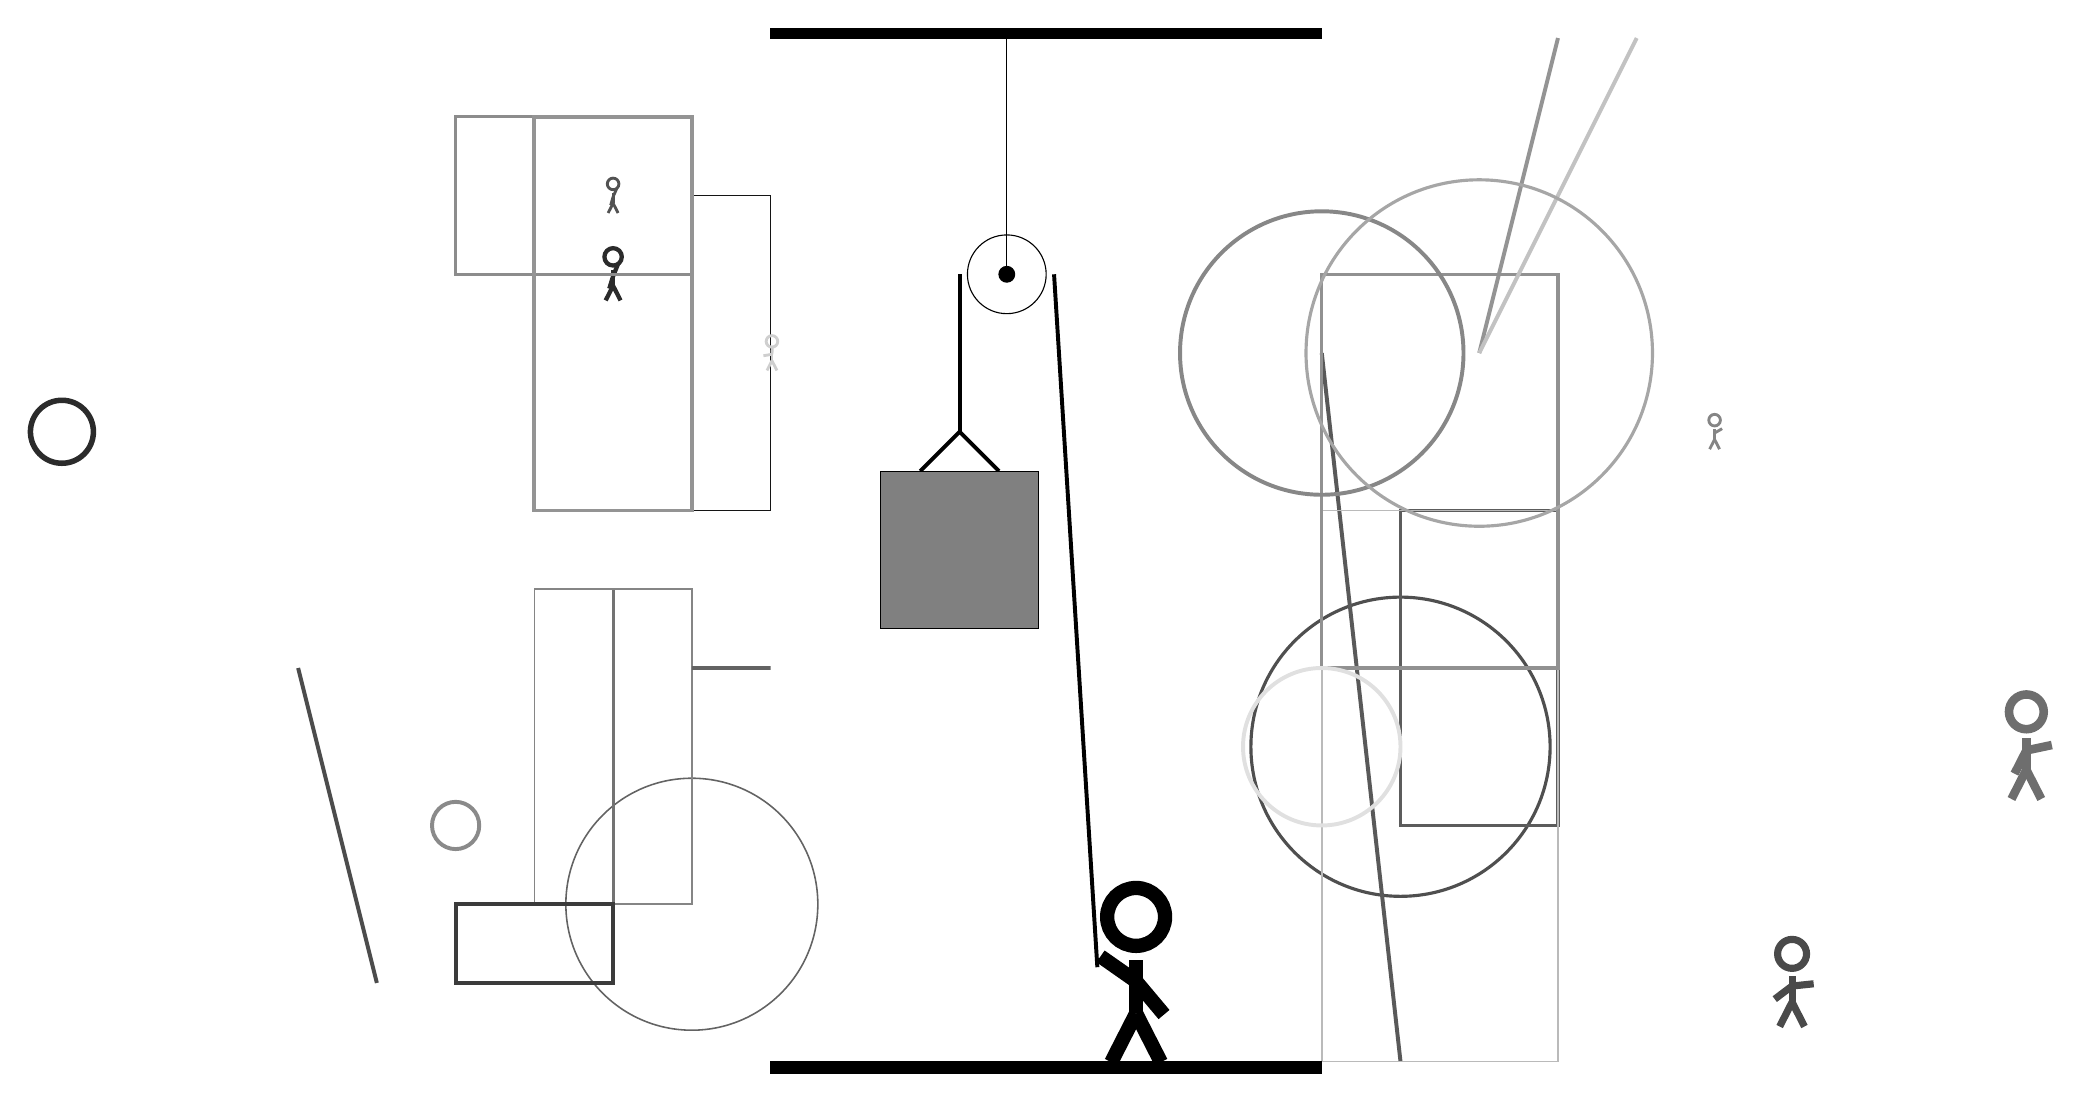
\begin{tikzpicture}
		%%%%% START %%%%%
		
		\draw[fill=black] (-2, 10) rectangle (5, 10.125);
		
		\node[line width=0.3mm, color=black!48] at (10, 5) {\Strichmaxerl[2][90][30]};
		
		\draw [line width=0.2mm, color=black!61](-3, -1) circle (1.6);
		\draw [line width=0.4mm, color=black!69](6, 1) circle (1.9);
		\draw[line width=0.2mm, color=black!60] (-3, 3) rectangle (-3, -1);
		\draw[line width=0.4mm, color=black!55] (-4, -1) rectangle (-4, 3);
		\node[line width=0.4mm, color=black!68] at (-4, 8) {\Strichmaxerl[2][74][66]};
		\node[line width=0.2mm, color=black!83] at (-4, 7) {\Strichmaxerl[3][73][68]};
		\draw[line width=0.5mm, color=black!70](-7, -2) -- (-8, 2);
		\draw[line width=0.2mm, color=black!48] (-3, -1) rectangle (-5, 3);
		\draw[line width=0.5mm, color=black!65](5, 6) -- (6, -3);
		
		\draw[line width=0.5mm, color=black!64] (6, 0) rectangle (8, 4);
		\draw[line width=0.5mm, color=black!42](7, 6) -- (8, 10);
		\node[line width=0.3mm, color=black!57] at (14, 1) {\Strichmaxerl[6][63][12]};
		\draw[line width=0.2mm, color=black!27] (5, 4) rectangle (8, -3);
		\draw[line width=0.4mm, color=black!43] (5, 7) rectangle (8, 2);
		\draw[line width=0.6mm, color=black!61] (-2, 2) rectangle (-3, 2);
		\draw[line width=0.5mm, color=black!77] (-4, -1) rectangle (-6, -2);
		\draw [line width=0.5mm, color=black!47](5, 6) circle (1.8);
		\draw[line width=0.2mm, color=black!92] (-3, 4) rectangle (-2, 8);
		\draw[line width=0.5mm, color=black!24](9, 10) -- (7, 6);
		\draw [line width=0.4mm, color=black!35](7, 6) circle (2.2);
		
		\draw [line width=0.5mm, color=black!12](5, 1) circle (1.0);
		\draw[line width=0.4mm, color=black!45] (-3, 7) rectangle (-6, 9);
		\draw[line width=0.5mm, color=black!42] (-3, 4) rectangle (-5, 9);
		\node[line width=0.4mm, color=black!19] at (-2, 6) {\Strichmaxerl[2][10][87]};
		
		\draw [line width=0.5mm, color=black!46](-6, 0) circle (0.3);
		\node[line width=0.3mm, color=black!71] at (11, -2) {\Strichmaxerl[5][37][6]};
		\draw [line width=0.7mm, color=black!83](-11, 5) circle (0.4);
		
		\draw (1, 7) circle (0.5);
		\draw[fill=black] (1, 7) circle (0.1);
		\draw (1, 10) -- (1, 7);
		
		\draw[line width=0.5mm] (-0.1, 4.5) -- (0.4, 5.0) -- (0.9, 4.5);
		\draw[fill=black!50] (-0.6, 4.5) rectangle (1.4, 2.5);
		
		\draw[line width=0.5mm] (0.4, 7) -- (0.4, 5.0);
		\centerarc[line width=0.5mm](1, 7)(0:180:0.6);
		\draw[line width=0.5mm](1.6, 7) -- (2.15, -1.8);
		
		\node at (2.6, -1.9) {\Strichmaxerl[10][-35][-50]};
		
		\draw[fill=black] (-2, -3) rectangle (5, -3.15);
		
		%%%%% END %%%%%
	\end{tikzpicture}
\end{document}